% Practice Test 14 — Indiana Edition
% Questions: 30 (21 MC + 9 SA)
% Generated by scripts/generate_practice_tests.py

\begin{practiceQuestion}{1-3-q02}{mc}
\begin{questionText}
In a proportional relationship, the constant of proportionality $k$ equals:
\end{questionText}
\choiceA{$x \div y$}
\choiceB{$y \div x$}
\choiceC{$x \times y$}
\choiceD{$y - x$}
\correctAnswer{B}
\explanation{The constant of proportionality is $k = \frac{y}{x}$, which is the unit rate.}
\end{practiceQuestion}

\begin{practiceQuestion}{1-5-q22}{sa}
\begin{questionText}
Explain what the point $(0, 0)$ means on a graph of cost versus number of books purchased.
\end{questionText}
\correctAnswer{Buying $0$ books costs $\$0$}
\explanation{The origin means both quantities are zero: zero books and zero cost. This confirms no fixed fee.}
\end{practiceQuestion}

\begin{practiceQuestion}{1-6-q08}{mc}
\begin{questionText}
A machine fills $350$ bottles in $5$ hours. How many bottles does it fill in $12$ hours?
\end{questionText}
\choiceA{$700$}
\choiceB{$780$}
\choiceC{$840$}
\choiceD{$900$}
\correctAnswer{C}
\explanation{Rate: $350 \div 5 = 70$ bottles/hr. In $12$ hours: $70 \times 12 = 840$ bottles.}
\end{practiceQuestion}

\begin{practiceQuestion}{2-2-q29}{gsa}
\begin{questionText}
The double number line below shows a percent relationship. What number goes at the question mark?

\begin{center}
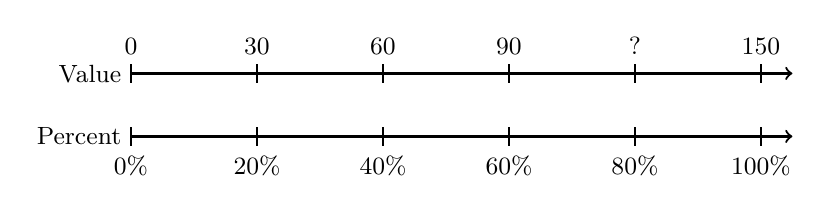
\begin{tikzpicture}[scale=0.8]
  % Top number line (values)
  \draw[thick,->] (0,1) -- (10.5,1);
  \node[left,font=\small] at (0,1) {Value};
  \foreach \x/\lab in {0/0, 2/30, 4/60, 6/90, 8/?, 10/150} {
    \draw[thick] (\x,0.85) -- (\x,1.15);
    \node[above,font=\small] at (\x,1.15) {\lab};
  }
  % Bottom number line (percent)
  \draw[thick,->] (0,0) -- (10.5,0);
  \node[left,font=\small] at (0,0) {Percent};
  \foreach \x/\lab in {0/0\%, 2/20\%, 4/40\%, 6/60\%, 8/80\%, 10/100\%} {
    \draw[thick] (\x,-0.15) -- (\x,0.15);
    \node[below,font=\small] at (\x,-0.15) {\lab};
  }
\end{tikzpicture}
\end{center}
\end{questionText}
\correctAnswer{$120$}
\explanation{The whole ($100\%$) corresponds to $150$. At $80\%$: $\frac{n}{150} = \frac{80}{100}$ → $n = 120$.}
\end{practiceQuestion}

\begin{practiceQuestion}{2-5-q29}{gsa}
\begin{questionText}
The receipt below shows a restaurant bill. Calculate the $18\%$ tip and the total amount.

\begin{center}
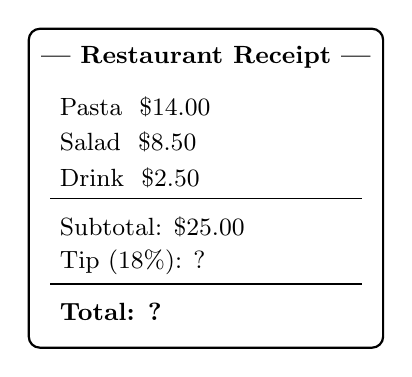
\begin{tikzpicture}[scale=0.9]
  \draw[thick,rounded corners] (0,0) rectangle (5,4.5);
  \node[font=\small\bfseries] at (2.5,4.1) {--- Restaurant Receipt ---};
  \node[anchor=west,font=\small] at (0.3,3.4) {Pasta \dotfill\ $\$14.00$};
  \node[anchor=west,font=\small] at (0.3,2.9) {Salad \dotfill\ $\$8.50$};
  \node[anchor=west,font=\small] at (0.3,2.4) {Drink \dotfill\ $\$2.50$};
  \draw[thin] (0.3,2.1) -- (4.7,2.1);
  \node[anchor=west,font=\small] at (0.3,1.7) {Subtotal: $\$25.00$};
  \node[anchor=west,font=\small] at (0.3,1.2) {Tip (18\%): ?};
  \draw[thick] (0.3,0.9) -- (4.7,0.9);
  \node[anchor=west,font=\small\bfseries] at (0.3,0.5) {Total: ?};
\end{tikzpicture}
\end{center}
\end{questionText}
\correctAnswer{Tip $= \$4.50$; Total $= \$29.50$}
\explanation{Tip: $25.00 \times 0.18 = \$4.50$. Total: $25.00 + 4.50 = \$29.50$.}
\end{practiceQuestion}

\begin{practiceQuestion}{2-7-q20}{sa}
\begin{questionText}
A student predicted a plant would grow $15$ cm. It actually grew $12$ cm. What is the percent error?
\end{questionText}
\correctAnswer{$25\%$}
\explanation{$\frac{|15 - 12|}{12} \times 100 = \frac{3}{12} \times 100 = 25\%$.}
\end{practiceQuestion}

\begin{practiceQuestion}{3-1-q22}{sa}
\begin{questionText}
A submarine is at $-200$ meters. It rises $200$ meters. What is its new depth?
\end{questionText}
\correctAnswer{$0$ meters (sea level)}
\explanation{$-200 + 200 = 0$. Rising $200$ meters from $-200$ meters brings the submarine to sea level.}
\end{practiceQuestion}

\begin{practiceQuestion}{3-2-q24}{sa}
\begin{questionText}
A football team has the following plays: gain $7$ yards, lose $3$ yards, lose $5$ yards, gain $2$ yards. What is the net yardage?
\end{questionText}
\correctAnswer{$1$ yard}
\explanation{$7 + (-3) + (-5) + 2 = 1$. Gains: $7 + 2 = 9$. Losses: $3 + 5 = 8$. Net: $9 - 8 = 1$ yard gained.}
\end{practiceQuestion}

\begin{practiceQuestion}{4-2-q18}{mc}
\begin{questionText}
A student says that $4x + 4y = 8xy$. Is the student correct?
\end{questionText}
\choiceA{Yes, because $4 + 4 = 8$ and the variables combine as $xy$.}
\choiceB{No, because $4x$ and $4y$ are not like terms and cannot be combined.}
\choiceC{Yes, because the coefficients are the same.}
\choiceD{No, because the answer should be $(4x)(4y) = 16xy$.}
\correctAnswer{B}
\explanation{$4x$ and $4y$ have different variables, so they are not like terms and cannot be combined. The expression $4x + 4y$ is already simplified.}
\end{practiceQuestion}

\begin{practiceQuestion}{4-3-q17}{mc}
\begin{questionText}
Expand $0.5(4x + 10)$.
\end{questionText}
\choiceA{$4.5x + 10.5$}
\choiceB{$2x + 5$}
\choiceC{$2x + 10$}
\choiceD{$4x + 5$}
\correctAnswer{B}
\explanation{$0.5 \times 4x = 2x$ and $0.5 \times 10 = 5$. Result: $2x + 5$.}
\end{practiceQuestion}

\begin{practiceQuestion}{5-4-q07}{mc}
\begin{questionText}
Solve $\dfrac{3n}{4} + 6 = 15$.
\end{questionText}
\choiceA{$n = 28$}
\choiceB{$n = 12$}
\choiceC{$n = 7$}
\choiceD{$n = 36$}
\correctAnswer{B}
\explanation{Subtract $6$: $\frac{3n}{4} = 9$. Multiply by $4$: $3n = 36$. Divide by $3$: $n = 12$. Check: $\frac{3(12)}{4} + 6 = 9 + 6 = 15$ \checkmark.}
\end{practiceQuestion}

\begin{practiceQuestion}{5-5-q06}{mc}
\begin{questionText}
Solve $-4x > 20$.
\end{questionText}
\choiceA{$x > -5$}
\choiceB{$x < -5$}
\choiceC{$x > 5$}
\choiceD{$x < 5$}
\correctAnswer{B}
\explanation{Divide by $-4$ and flip the sign: $x < -5$.}
\end{practiceQuestion}

\begin{practiceQuestion}{5-6-q28}{gmc}
\begin{questionText}
Look at the two number lines below. Which statement is true?

\textbf{Line 1:}
\begin{center}
\begin{tikzpicture}[scale=0.55]
  \draw[thick,->] (-6,0) -- (6,0);
  \foreach \x in {-5,...,5} \draw (\x,0.12) -- (\x,-0.12) node[below,font=\small] {$\x$};
  \draw[thick,funBlue,->] (-3,0) -- (6,0);
  \fill[funBlue] (-3,0) circle (4pt);
\end{tikzpicture}
\end{center}

\textbf{Line 2:}
\begin{center}
\begin{tikzpicture}[scale=0.55]
  \draw[thick,->] (-6,0) -- (6,0);
  \foreach \x in {-5,...,5} \draw (\x,0.12) -- (\x,-0.12) node[below,font=\small] {$\x$};
  \draw[thick,funOrange,->] (-3,0) -- (6,0);
  \draw[thick,funOrange,fill=white] (-3,0) circle (4pt);
\end{tikzpicture}
\end{center}
\end{questionText}
\choiceA{Both graphs include $-3$ as a solution}
\choiceB{Line 1 shows $x \geq -3$ and Line 2 shows $x > -3$}
\choiceC{Line 1 shows $x > -3$ and Line 2 shows $x \geq -3$}
\choiceD{Both graphs represent the same inequality}
\correctAnswer{B}
\explanation{Line 1 has a closed circle (includes $-3$): $x \geq -3$. Line 2 has an open circle (excludes $-3$): $x > -3$.}
\end{practiceQuestion}

\begin{practiceQuestion}{6-1-q04}{mc}
\begin{questionText}
On a map, $2$ cm represents $50$ km. What is the scale factor?
\end{questionText}
\choiceA{$2$ km per cm}
\choiceB{$25$ km per cm}
\choiceC{$50$ km per cm}
\choiceD{$100$ km per cm}
\correctAnswer{B}
\explanation{Find the unit rate: $50 \div 2 = 25$ km per cm.}
\end{practiceQuestion}

\begin{practiceQuestion}{6-3-q01}{mc}
\begin{questionText}
Can you draw a triangle with sides $3$ cm, $4$ cm, and $8$ cm?
\end{questionText}
\choiceA{Yes, and it is a unique triangle}
\choiceB{Yes, and more than one triangle is possible}
\choiceC{No, because the angles don't add to $180°$}
\choiceD{No, because $3 + 4 < 8$}
\correctAnswer{D}
\explanation{The triangle inequality requires the sum of any two sides to be greater than the third. Here $3 + 4 = 7 < 8$, so no triangle can be formed.}
\end{practiceQuestion}

\begin{practiceQuestion}{6-4-q03}{mc}
\begin{questionText}
Can a triangle have angles $50°$, $60°$, and $80°$?
\end{questionText}
\choiceA{Yes, because the angles are all positive}
\choiceB{Yes, because each angle is less than $180°$}
\choiceC{No, because $50 + 60 + 80 = 190 \neq 180$}
\choiceD{No, because the angles are not equal}
\correctAnswer{C}
\explanation{The three angles sum to $190°$, not $180°$. Triangle angles must always sum to exactly $180°$.}
\end{practiceQuestion}

\begin{practiceQuestion}{6-5-q17}{mc}
\begin{questionText}
A triangular prism is sliced with a vertical cut perpendicular to the triangular bases. What shape is the cross-section?
\end{questionText}
\choiceA{Triangle}
\choiceB{Rectangle}
\choiceC{Circle}
\choiceD{Trapezoid}
\correctAnswer{B}
\explanation{A vertical cut perpendicular to the triangular bases of a triangular prism produces a rectangle (the cut goes through the lateral faces).}
\end{practiceQuestion}

\begin{practiceQuestion}{6-6-q26}{gmc}
\begin{questionText}
Two lines intersect as shown. What is the value of $x$?

\begin{center}
\begin{tikzpicture}[scale=0.8]
  \draw[thick] (-3,0) -- (3,0);
  \draw[thick] (-2,-2) -- (2,2);
  \node at (1.5,0.5) {\small $x°$};
  \node at (-1.5,-0.6) {\small $x°$};
  \node at (-1.2,0.8) {\small $135°$};
\end{tikzpicture}
\end{center}
\end{questionText}
\choiceA{$35°$}
\choiceB{$45°$}
\choiceC{$55°$}
\choiceD{$135°$}
\correctAnswer{B}
\explanation{The angle $x°$ and $135°$ are supplementary (they are adjacent on a straight line): $x + 135 = 180$. So $x = 45°$.}
\end{practiceQuestion}

\begin{practiceQuestion}{6-7-q12}{mc}
\begin{questionText}
Point $J(6, -2)$ is rotated $90°$ clockwise about the origin. What are the coordinates of $J'$?
\end{questionText}
\choiceA{$(2, 6)$}
\choiceB{$(-2, -6)$}
\choiceC{$(-6, 2)$}
\choiceD{$(-2, 6)$}
\correctAnswer{B}
\explanation{$90°$ clockwise: $(x, y) \to (y, -x)$. $(6, -2) \to (-2, -6)$.}
\end{practiceQuestion}

\begin{practiceQuestion}{7-3-q20}{sa}
\begin{questionText}
A circular garden has a diameter of $20$ meters. What is its area? Use $\pi \approx 3.14$.
\end{questionText}
\correctAnswer{$314$ m$^2$}
\explanation{$r = 10$ m. $A = \pi r^2 = 3.14 \times 100 = 314$ m$^2$.}
\end{practiceQuestion}

\begin{practiceQuestion}{7-4-q06}{mc}
\begin{questionText}
An L-shaped room can be split into a $10$ ft by $8$ ft rectangle and a $4$ ft by $6$ ft rectangle. What is the total floor area?
\end{questionText}
\choiceA{$56$ ft$^2$}
\choiceB{$80$ ft$^2$}
\choiceC{$104$ ft$^2$}
\choiceD{$128$ ft$^2$}
\correctAnswer{C}
\explanation{$10 \times 8 = 80$ ft$^2$. $4 \times 6 = 24$ ft$^2$. Total: $80 + 24 = 104$ ft$^2$.}
\end{practiceQuestion}

\begin{practiceQuestion}{7-5-q22}{sa}
\begin{questionText}
A cube has a surface area of $384$ in$^2$. What is the side length?
\end{questionText}
\correctAnswer{$8$ in}
\explanation{$s^2 = 384 \div 6 = 64$. So $s = 8$ in.}
\end{practiceQuestion}

\begin{practiceQuestion}{7-6-q28}{gmc}
\begin{questionText}
A triangular prism is shown below. What is its volume?

\begin{center}
\begin{tikzpicture}[scale=0.35]
  % Front triangle
  \fill[funBlue!10] (0,0) -- (8,0) -- (4,5) -- cycle;
  \draw[thick,funBlue] (0,0) -- (8,0) -- (4,5) -- cycle;
  % Back triangle
  \fill[funBlue!20] (3,2) -- (11,2) -- (7,7) -- cycle;
  \draw[thick,funBlue] (3,2) -- (11,2) -- (7,7) -- cycle;
  % Connecting edges
  \draw[thick,funBlue] (0,0) -- (3,2);
  \draw[thick,funBlue] (8,0) -- (11,2);
  \draw[thick,funBlue] (4,5) -- (7,7);
  % Labels
  \draw[thick,funRed,<->] (0,-0.8) -- (8,-0.8);
  \node[below,funRed] at (4,-0.8) {$8$ m};
  \draw[dashed,gray] (4,0) -- (4,5);
  \node[left,funRed] at (3.8,2.5) {$5$ m};
  \node[right,funRed] at (11.2,4.5) {$12$ m};
\end{tikzpicture}
\end{center}
\end{questionText}
\choiceA{$120$ m$^3$}
\choiceB{$240$ m$^3$}
\choiceC{$480$ m$^3$}
\choiceD{$96$ m$^3$}
\correctAnswer{B}
\explanation{$B = \frac{1}{2} \times 8 \times 5 = 20$ m$^2$. $V = 20 \times 12 = 240$ m$^3$.}
\end{practiceQuestion}

\begin{practiceQuestion}{8-1-q06}{mc}
\begin{questionText}
A city wants to survey residents about a new park. Which method would produce the least biased sample?
\end{questionText}
\choiceA{Survey people at the existing park}
\choiceB{Put the survey in the newspaper and wait for responses}
\choiceC{Randomly select addresses from the city directory}
\choiceD{Survey people at the city council meeting}
\correctAnswer{C}
\explanation{Randomly selecting addresses gives all residents an equal chance, reducing bias.}
\end{practiceQuestion}

\begin{practiceQuestion}{8-3-q25}{sa}
\begin{questionText}
Two groups have means of $50$ and $54$, and both have MAD $= 8$. Express the difference in means as a multiple of MAD. Is the difference meaningful?
\end{questionText}
\correctAnswer{$0.5$ MADs; no, the difference is not meaningful}
\explanation{$\frac{54-50}{8} = 0.5$ MADs. Since $0.5 < 2$, the difference is small relative to the variability and not considered meaningful.}
\end{practiceQuestion}

\begin{practiceQuestion}{8-4-q27}{gmc}
\begin{questionText}
The box plots show quiz scores (out of $20$) for two classes.

\begin{center}
\begin{tikzpicture}[scale=0.35]
  \draw[thick,->] (4,0) -- (21,0);
  \foreach \x in {5,6,...,20} {
    \draw (\x,0.3) -- (\x,-0.3);
    \node[below,font=\tiny] at (\x,-0.3) {$\x$};
  }
  % Class M: min=8, Q1=12, med=15, Q3=17, max=20
  \draw[thick] (8,3) -- (20,3);
  \draw[thick,fill=funBlue!30] (12,2) rectangle (17,4);
  \draw[very thick,funBlue] (15,2) -- (15,4);
  \draw[thick] (8,2) -- (8,4);
  \draw[thick] (20,2) -- (20,4);
  \node[right,font=\small] at (20.5,3) {Class M};
  % Class N: min=10, Q1=13, med=16, Q3=18, max=19
  \draw[thick] (10,7) -- (19,7);
  \draw[thick,fill=funGreen!30] (13,6) rectangle (18,8);
  \draw[very thick,funGreen] (16,6) -- (16,8);
  \draw[thick] (10,6) -- (10,8);
  \draw[thick] (19,6) -- (19,8);
  \node[right,font=\small] at (19.5,7) {Class N};
\end{tikzpicture}
\end{center}

What is the IQR for each class?
\end{questionText}
\choiceA{Class M: $5$, Class N: $5$}
\choiceB{Class M: $12$, Class N: $9$}
\choiceC{Class M: $5$, Class N: $9$}
\choiceD{Class M: $12$, Class N: $5$}
\correctAnswer{A}
\explanation{Class M: $Q_3 - Q_1 = 17 - 12 = 5$. Class N: $18 - 13 = 5$. Both have IQR $= 5$.}
\end{practiceQuestion}

\begin{practiceQuestion}{8-7-q09}{mc}
\begin{questionText}
Which display is best for comparing exact frequencies of categorical data?
\end{questionText}
\choiceA{Line graph}
\choiceB{Frequency table}
\choiceC{Box plot}
\choiceD{Dot plot}
\correctAnswer{B}
\explanation{A frequency table lists exact counts for each category, which is ideal for comparing categorical data.}
\end{practiceQuestion}

\begin{practiceQuestion}{9-4-q16}{mc}
\begin{questionText}
A game has $4$ outcomes: Win Big, Win Small, Lose Small, Lose Big. The probabilities are $0.05$, $0.25$, $0.45$, and $0.25$. Which outcome is LEAST likely?
\end{questionText}
\choiceA{Win Big}
\choiceB{Win Small}
\choiceC{Lose Small}
\choiceD{Lose Big}
\correctAnswer{A}
\explanation{Win Big has the smallest probability ($0.05$), making it least likely.}
\end{practiceQuestion}

\begin{practiceQuestion}{9-6-q11}{mc}
\begin{questionText}
Two dice are rolled. What is the probability that the sum is even?
\end{questionText}
\choiceA{$\frac{1}{4}$}
\choiceB{$\frac{1}{3}$}
\choiceC{$\frac{1}{2}$}
\choiceD{$\frac{2}{3}$}
\correctAnswer{C}
\explanation{Even sums occur when both dice are even or both are odd. Both even: $3 \times 3 = 9$. Both odd: $3 \times 3 = 9$. Total: $18$ out of $36$. $P = \frac{18}{36} = \frac{1}{2}$.}
\end{practiceQuestion}

\begin{practiceQuestion}{9-7-q03}{mc}
\begin{questionText}
To simulate an event with a $\frac{1}{6}$ probability, which tool would be most appropriate?
\end{questionText}
\choiceA{A coin}
\choiceB{A standard die}
\choiceC{A spinner with $4$ sections}
\choiceD{A bag with $2$ marbles}
\correctAnswer{B}
\explanation{A standard die has $6$ equally likely outcomes, each with probability $\frac{1}{6}$.}
\end{practiceQuestion}
